% Chapter 1

\chapter{Numerical Methods for Phase Change Phenomena} % Main chapter title

\label{Chapter2} % For referencing the chapter elsewhere, use \ref{Chapter1} 

%----------------------------------------------------------------------------------------

% Define some commands to keep the formatting separated from the content 
\section{State of Art. Numerical Methods} %Description of general numerical methods for phase change 
\setlength{\parindent}{0.5cm} Considering the PCM density as constant in the model might be thought as a reasonable assumption in some cases, in others where thermo-mechanical coupling between the fluid and its container is intended, it makes impossible to account for some physical behaviors which may result from expansion or contraction during the phase change of the material. However, the main goal of this thesis is not to present a method that represents thermo-mechanical coupling but a technique that ensures volume expansion due to density changes through the fluid domain.
To reach this point, it is important to summarize some of the numerous researches that have been conducted in order to investigate the problem of solidification. 

\noindent At the present, the main used numerical methods representing the treatment of liquid-solid phase change are divided into these categories:
\begin{itemize}
	\item \textbf{Front tracking method},
	\subitem \textbf{Volume-of-fluid method},
	\subitem \textbf{Level set method},
	\item \textbf{Enthalpy method},
	\item \textbf{Phase field method}.
\end{itemize}

\subsection{Front tracking method}

\setlength{\parindent}{0.5cm} Several studies are carried out with this method. Juric et al. \cite{juric_tryggvason_1996}, presented a front-tracking method based on a finite difference approach of the heat equation and an explicit tracking of the fluid-solid interface to simulate time dependent two-dimensional dendritic solidification of pure substances. In similar fields, Al-Rawahi et al. \cite{al-rawahi_tryggvason_2002} underwent also simulations of dendritic growth of pure substances by using front-tracking methods in which the fluid-solid interface was tracked explicitly and the release of latent heat during solidification was calculated with the normal temperature gradient near the interface. Accordingly, Garimella et al. \cite{li_garimella_simpson_2003} proposed an explicit interface-tracking scheme involving reconstruction and advection of the moving interface in a fixed grid to solve moving-boundary problems associated with phase change phenomena. As they describe, the movement of the interface is tackled first by advection and tracking of the interface, later by the calculation of normal velocities near the interface region and finally, by solving the governing equations for the existing phases.

\subsection*{Volume-of-fluid method}

\setlength{\parindent}{0.5cm} Initially introduced by Harlow et al. \cite{harlow_welch_1965}, a technique called the marker and cell method tracked the interface by wightless particles which were transported convectively by the velocity of the fluid. Cells that were filled with marked particles were considered occupied by the fluid while, contrarily, these which were not filled with marked particles were not occupied by fluid. Later in time, the idea was extended to track the interface based on phase fractions in the volume-of-fluid method which is discussed in detail later in this chapter.

\subsection*{Level set method}

\setlength{\parindent}{0.5cm} In the field of the current technique, Tan et al. \cite{tan_zabaras_2007} conducted a level set method combining properties of both fixed domain and front-tracking methods to model the microstructure evolution in multi-component alloy solidification. Phase interface is tracked by solving the multi-phase level set equations. From this tracked interface, a diffused one is constructed by means of the level set functions. Volume-averaging methods are latter used to solve energy, species and momentum equations.  Rauschenberger et al. \cite{rauschenberger_criscione_eisenschmidt_kintea_jakirlic_tukovic_roisman_weigand_tropea_2013} pursued a comparative assessment between a Level set approach and a volume-of-fluid method to track interfaces in the context of dendritic ice growth in supercooled water. The Level Set method is used as an implicit tracking of the moving boundary.

\subsection{Enthalpy method}

\setlength{\parindent}{0.5cm} In 2004, Esen et al. \cite{esen_kutluay_2004} worked out an enthalpy method based on finite difference approximations applied to the Stefan problem. An enthalpy function is defined representing the total heat content per unit of mass of the material. The need of tracking the interface between the fluid and the solid phase is thereby removed when using such formulation. El Ganaoui et al. \cite{el_ganaoui_lamazouade_bontoux_morvan_2002} presented an enthalpy-porosity formulation on a fixed grid framework for liquid-to-solid phase transition. The method is extended to solve time-dependent solutal convection in the melt during directional solidification that undergo the majority of alloys. Within the alloy research field, Voller et al. \cite{voller_2008} developed an enthalpy fixed grid method for dendritic growth modeling in under-cooled binary alloys. This method is devoted to couple explicit finite differences expressing the conservation of enthalpy and solute to an iterative scheme which enforces node-to-node consistency between solute, liquid-fraction, enthalpy and under-cooling interface.

\subsection{Phase field method}

\setlength{\parindent}{0.5cm} Emerged as an approach to model and predict mesoscale morphological and microstructure evolution in materials, Chen et al. \cite{chen_2002} review some phase-field models used to describe various materials processes including solidification, crack propagation and dislocation microstructures among others. This paper describes the capability of phase-field methods to predict the evolution of arbirtary morphologies and complex microstructures without explicitly tracking the evolution of the interface.

\section{Solidification methods}

\setlength{\parindent}{0.5cm} The challenge of a numerical investigation of a solidification process is to capture the free surface for the flow of the phase change material and, at the same time, account for the moving boundary induced by the phase change within the PCM. The free surface may be handled by the volume-of-fluid (VOF), originally introduced by Hirt and Nichols  \cite{hirt_nichols_1981}. VOF relies on the definition of a transport indicator function within the finite volume method's framework.

\noindent Simultaneously, and in order to account for the phase changes, some of the used models are based on meso-scale. This is the phenomena occurring between microscopic and continuum length scales and, in the current context, the complex micro structure generated during the solidification is approximated as liquid, mushy (intermediate state), and solid regions. Mushy region is thereby described as an averaged value of the liquid and solid properties.

\noindent One of the most used methods is the enthalpy-porosity technique, originally developed by Voller and Prakash \cite{voller_prakash_1987}, which uses the typical conservation equations on a fixed Eulerian grid. The main concepts underlaying such method are: on the one side, an additional source term to the energy conservation equation is applied to describe the release of latent heat. On the other side, the solidification effects on the mass transport are modelled as a porosity variable and this is introduced as a Darcy-type source term to the momentum equation.


\noindent In the first aim of this thesis is the coupled use of the enthalpy-porosity technique with the VOF method. Some of the studies found on this topic, the coupling of both VOF and enthalpy-porosity methods, are mainly related to casting processes. Rösler and Brüggermann \cite{rösler_brüggemann_2011} introduced a numerical model for a solid-liquid phase change inside a latent heat thermal energy storage. Richter et al. \cite{richter_turnow_kornev_hassel_2016}, worked out a method for the simultaneous mould filling and solidification process which settles the developing of free surface flow and the liquid-solid phase transition under the volume-of-fluid and enthalpy-porosity methods.

\noindent However, no adaptation of these methods to purely solidification processes has been found. Therefore, the objectives of the first stage of the research are:
\begin{itemize}
	\item To introduce a new solver based on the coupling of VOF and enthalpy-porosity techniques which covers the relevant physical effects during the process of solidification.
	\item	To validate simulation results by using benchmark cases found in the literature.
\end{itemize}
Numerical methods commented here are deeply described next.

\subsection{Volume-of-Fluid Method: General Aspects}
\setlength{\parindent}{0.5cm} The Volume-of-fluid method (VOF) is a numerical method based on an Eulerian approach to track the free surface in a two-phase flow.
The VOF method, developed by Hirt and Nichols in 1981, \cite{hirt_nichols_1981}, takes relevance when fluids coexist with other phases. An example could be the ice (solid phase) advancing front within the liquid phase. The surface in between both phases needs to be solved by means of the volume of fluid technique.

\noindent This is sometimes seen as the conservation of the mixture components along the path of a fluid region. The equation which allows that is described as:
\begin{equation}
	\frac{\partial \alpha_{\text {phase }}}{\partial t}+\frac{\partial\left(\alpha_{\text {phase }} u_{j}\right)}{\partial x_{j}}=0
	\label{2.1}
\end{equation}
In which $\alpha_{phase}$ corresponds to the phase fraction and it applies:
\begin{equation}
	\alpha_{phase}= \begin{cases}
		0 & =\text { solid PCM } \\ 0<\alpha_{phase}<1 & =\text { cell contains the interface } \\ 1 & =\text { liquid } \mathrm{PCM}
	\end{cases}
	\label{2.2}
\end{equation}
\clearpage
\noindent As Eq. \ref{2.1} exposes, the principle that lies behind the method is the definition of the phase field ($\alpha$), Eq. \ref{2.2}, which has a value between '0' and '1'. The value of '1' corresponds to any point filled with fluid and zero, otherwise. Thus, the average value of $\alpha$	in a cell indicates the fractional volume of that cell occupied by the fluid. Consequently, if a cell has an average value of $\alpha=1$ implies a fully filled cell of fluid and oppositely, a value of $\alpha=0$ means that the fluid is not present in the cell. However, a cell presenting an average value between 0 and 1 would lead the presence of an interface in that region as it is clearly seen in Fig. \ref{2.1}.
\begin{figure}[h!]
	\centering
	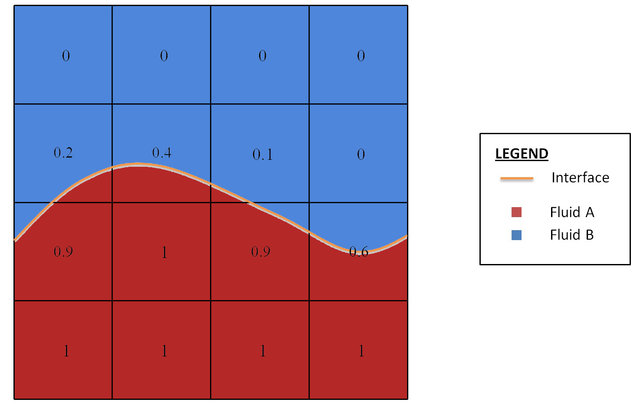
\includegraphics[width=.55\linewidth]{Volume-of-Fluid-approach.jpg}	
	\label{2.1fig}
	\caption{Volume-of-fluid approach.}
\end{figure} 

\noindent Near the interface, it clearly exists a jump in the fluid properties that need to be corrected by properly averaging phase properties in that region.

\noindent In the present study, this method is used in conjunction with other techniques to carry out some cases undergoing phase-transition phenomena.

\subsection{Enthalpy-Porosity Model. Governing Equations}

\setlength{\parindent}{0.5cm} The first technique implemented is the Enthalpy-porosity method. Here, the energy equation takes center stage. 

\noindent The energy equation based on the enthalpy formulation for convective-diffusive heat transfer states that,
\begin{equation}
	\frac{\partial \rho h}{\partial t}+\frac{\partial}{\partial x_{j}}\left(\rho u_{j} h\right)=\nabla \cdot\left(k_{i} \nabla T_{i}\right)
	\label{2.3}
\end{equation}

\noindent where \textit{u} is the velocity component and $\kappa_{i}$ is the thermal conductivity of the fluid.

\noindent However, the enthalpy-porosity method describes the enthalpy \textit{h} of the mixture by its sensible part and the latent heat of solidification.
The release of the latent heat is dependent on the stage of the phase change, and must be restricted to the phase change material.
\begin{equation}
	h=\int_{T_{r}}^{T} c_{p} d T+\alpha_{\ell} L
	\label{2.4}
\end{equation}
where the latent heat is is driven by the evolution of the liquid $\alpha_{l}$. The phase transition is modelled by expressing the liquid volume fraction as a function of the temperature,
\begin{equation}
	\alpha_{l}= \begin{cases}
		1 & T>T_{l i q} \\ \frac{T-T_{\text {sol }}}{T_{\text {liq }}-T_{\text {sol }}+\varepsilon} & T_{\text {sol }}<T<T_{l i q} \\ 0 & T<T_{\text {sol }}
	\end{cases}
	\label{2.5}
\end{equation}
For seek of brevity on the following expressions, it is adapted the term $\alpha_{phase}$ to $\alpha_{l}$ 
If expression \ref{2.5} is replaced in \ref{2.4},
\begin{equation}
	\begin{aligned}
		&\frac{\partial\left(\rho c_{p} T + \alpha_{l} L\right)}{\partial t}+\frac{\partial\left(\rho u_{j} c_{p} T + u_{j} \alpha_{l} L\right)}{\partial x_{j}} \\
		&=\nabla \cdot\left(k_{i} \nabla T_{i}\right)
	\end{aligned}
	\label{2.6}
\end{equation}
Rearranging terms, it yields the complete energy equation with the sensible and latent heat parts for the correct representation of solidification processes.
\begin{equation}
	\begin{aligned}
		\frac{\partial (\rho C_{p} T)}{\partial t}+ \nabla \cdot\left(u_{j}\rho C_{p} T\right)+L\left[\frac{\partial (\rho \alpha_{l})}{\partial t}+ \frac{\partial (u_{j}\rho \alpha_{l})}{\partial x_{j}}\right]=\nabla \cdot\left(k_{i} \nabla T_{i}\right)  \\
		S = -L\left[\frac{\partial (\rho \alpha_{l})}{\partial t}+ \frac{\partial (u_{j}\rho \alpha_{l})}{\partial x_{j}}\right]
	\end{aligned}
	\label{2.7}
\end{equation}
The momentum equation is discussed in detail in the sub-chapter \textit{Interphase porosity models}.

\subsection{Lee model}

\setlength{\parindent}{0.5cm} The second technique implemented in this thesis is based on the Lee model.

\noindent The Lee model is based in the liquid-vapour mass transfer. Governed by the vapour transport equation \ref{2.8}, this model is applicable during melting or solidification of a fluid.
\begin{equation}
	\frac{\partial}{\partial t}\left(\alpha_{i} \rho_{i}\right)+\nabla\left(\alpha_{i} \rho_{i} {u}_{i}\right)=S_{m _i}
	\label{2.8}
\end{equation}
\textit{$\rho_i$} and \textbf{$u_i$} are the fluid density and fluid velocity of the \textit{i{th}} phase. Moreover, $S_{m_i}$ is the mass source which takes on a zero value at the interface.

\noindent During melting, $T_l$ > $T_{sat}$,
\begin{equation}
	\frac{d m_{s l}}{d t}=C_{f} \rho_{s} \alpha_{s}\left(\frac{T_{s}-T_{s a t}}{T_{s a t}}\right)
	\label{2.9}
\end{equation}
During solidification, $T_l$ < $T_sat$
\begin{equation}
	\label{2.10}
	\frac{d m_{l s}}{d t}=C_{f} \rho_{l} \alpha_{l}\left(\frac{T_{s a t}-T_{l}}{T_{s a t}}\right)
\end{equation}
The coefficient $C_f$ might be interpreted as a time rate and must be empirically tunned. Its magnitude is expressed in $\frac{1}{s}$. $\alpha$ represents the phase volume fraction. $\frac{d m_{i}}{d t}$ are the mass transfer rates from one phase to another. The subscripts \textit{"s"}, \textit{"l"}, refer to solid and liquid phases respectively. \textit{$T_{sat}$}, is the phase transition temperature which, in case of pure water would be 273.15 K.
The source term of \ref{2.8} is then calculated as,
\begin{equation}
	\label{2.11}
	S_{m_{i}}=\left\{\begin{array}{lr}
	\frac{d m_{s l}}{d t}-\frac{d m_{l s}}{d t}, & \text { for water phase } \\
	\frac{d m_{l s}}{d t}-\frac{d m_{s l}}{d t}, & \text { for ice phase }
	\end{array}\right.
\end{equation}  

\subsubsection{Momentum Equation}

\setlength{\parindent}{0.5cm} In the momentum equation, the flow is modelled as,
\begin{equation}
	\label{2.12}
	\begin{aligned}
	&\frac{\partial\left(\rho {u}_{i}\right)}{\partial t}+\frac{\partial\left(\rho {u}_{i} {u}_{j}\right)}{\partial x_{j}} \\
	&\quad=-\alpha_{i} \nabla p+\frac{\partial}{\partial x_{j}}\left(\mu \frac{\partial {u}_{i}}{\partial x_{j}}\right)+F_{\sigma i}+S_{u_{i}}
	\end{aligned}
\end{equation}
The source term for the momentum equation can be written as,
\begin{equation}
	\label{2.13}
	S_{u_{i}}=\left\{\begin{array}{cr}
	\frac{d m_{s l}}{d t} \textbf{$u_{l}$}-\frac{d m_{l s}}{d t} \textbf{$u_{s},$} & \text { for water phase } \\
	\frac{d m_{l s}}{d t} \textbf{$u_{s}$}-\frac{d m_{s l}}{d t} \textbf{$u_{l}$}, & \text { for ice phase }
	\end{array}\right.
\end{equation}
where \textbf{$u_{l}$} and \textbf{$u_{s}$} are the liquid and solid velocity components accordingly. 

\noindent The source terms related to interphase porosity (\ref{2.29}) may be added to the momentum equation presented here for the Lee model \ref{2.12}.

\subsubsection{Energy Equation}

\setlength{\parindent}{0.5cm} The energy equation for the Lee model can be described as,
\begin{equation}
	\label{2.14}
	\frac{\partial (\rho C_{p} T)}{\partial t}+\nabla \cdot\left(u_{j}\rho C_{p} T\right)=\nabla \cdot\left(k_{i} \nabla T_{i}\right)+S_{H_{i}}
\end{equation}
where the heat source term due to mass transfer in the energy equation is calculated as,
\begin{equation}
	\label{2.15}
	S_{h_{i}}=\left\{\begin{array}{lr}
	\frac{d m_{s l}}{d t} H_{L,} & \text { for water phase } \\
	\frac{d m_{l s}}{d t} H_{L} & \text { for ice phase }
	\end{array}\right.
\end{equation}
where \textit{$H_l$} is the latent heat induced by the phase transition and \textit{$k_i$}, the thermal conductivity.

\subsubsection{Classical nucleation theory. The coefficient $C_f$.}

\setlength{\parindent}{0.5cm} The coefficient $C_f$ that appears on Equations \ref{2.9} and \ref{2.10} is computed accordingly to the work of Huang et al. \cite{huang_wang_li_2020}. In these work, the Lee model is used and the nucleation rate is introduced for the calculation of mass transfer rate between phases. 

\noindent The concept behind the \textit{Classical Nucleation Theory}, CNT, as described in \cite{ickes_welti_hoose_lohmann_2015} resides in the idea of droplet freezing. This is initiated in the fluctuation of molecules of a supercooled liquid due to thermal vibration which lead, at its turn, to spontaneous formation of ordered solid molecule clusters (ice embryos). The size of these embryos oscillates as individual water molecules are crystallized or lost from the liquid phase. When the size of the embryo reaches a critical value, it leads a faster and auspicious thermodynamic joining of further water molecules to the crystal lattice. This means the critical embryo enhancing the "parent phase", supercooled liquid, to undergo a macroscopic phase transition: droplet freezing.

\noindent And this is what CNT aims to describe; the freezing process in terms of temperature-dependent nucleation rate by joining two components: thermodynamic and kinetic. These components, briefly described in the following chapters, are based on the theory found in Lai et al. \cite{wu_lai_zhang_2015} and Huang et al. \cite{huang_wang_li_2020}.

\noindent As a remark, in this thesis a brief introduction of this theory is given. However, for further details on the assumptions used refer to the literature.

\subsubsection*{Thermodynamic component}

\setlength{\parindent}{0.5cm} This thermodynamic component seeks for the number of critical embryos formed per unit of volume at a specific temperature. A decrease in the enthalpy, and consequently a change in Gibbs free energy required to form an ice embryo containing water molecules generates an energy barrier to nucleation. However, for ice embryo formation, this barrier needs to be overcome. 
\begin{equation}
	\label{2.16}
	\Delta G_{c}=\underbrace{\Delta G_{V}}_{\text {volume term }}+\underbrace{\Delta G_{S}}_{\text {surface term }}
\end{equation}
where the volume and surface terms decomposed,
\begin{equation}
	\label{2.17}
	\Delta G_{c}=-\frac{4}{3} \cdot \frac{\pi r^{3}}{\Omega} \cdot \Delta g_{v}+4 \pi r^{2} \gamma_{s f}
\end{equation}
where $r$ is the radius of a simplified spherical embryo, $\gamma_{sf}$ the interfacial tension between phases $\Omega$ the volume of a single molecule $
\left(\Omega=V_{m, w} / N_{A}\right)$, $V_{m, w}$ is the molar volume and $\Delta g_{v}$ represents the decrease in volume of the Gibbs free energy of a molecule and is defined as:
\begin{equation}
	\label{2.18}
	\Delta g_{v}=\frac{\Delta_{m} H_{1}}{N_{A}} \frac{\Delta T}{T^{*}}
\end{equation}
where $\Delta_{m} H_{1}$ is the molar latent heat of crystallization, $N_{A}$ is the Avogadro's number, $T^{*}$ is the freezing temperature and $\delta T=T^* - T$, the degree of supercooling.
The radius has an influence on the change in Gibbs free energy. This is when:
\begin{itemize}
	\item $r < r_{crit} \Rightarrow \Delta G_{c} > 0 \hspace{0.25cm} || \hspace{0.25cm} \Delta G_{c} \uparrow \hspace{0.25cm} \Rightarrow \hspace{0.25cm} r \uparrow $ $\Leftarrow$ endothermic process
	\item $r > r_{crit} \Rightarrow \Delta G_{c} < 0 \hspace{0.25cm} || \hspace{0.25cm} \Delta G_{c} \downarrow \hspace{0.25cm} \Rightarrow \hspace{0.25cm} r \uparrow $ $\Leftarrow$ exothermic process
\end{itemize}
The critical radius exists when the global enthalpy variation gets negative.

\noindent By differentiating Eq. \ref{2.17} and setting $\frac{d(\Delta G_c)}{dr} = 0$, the critical radius is defined as:
\begin{equation}
	\label{2.19}
	r_{c r i t}=\frac{2 \gamma_{s f} T^{*} V_{m, w}}{\Delta_{m} H_{1} \Delta T}
\end{equation}
Then, if subsituting Eq. \ref{2.18} and \ref{2.19} in Eq. \ref{2.17}, it is obtained the energy barrier:
\begin{equation}
	\label{2.20}
	\Delta G_{c r i t}=\frac{16 \pi}{3} \cdot \frac{\gamma_{s f}^{3} V_{m, w}^{2} T^{2}}{\Delta_{m} H_{1}^{2} \Delta T^{2}}=\frac{1}{3}\left(4 \pi r_{c r i t}^{2} \gamma_{s f}\right)
\end{equation}
In Huang et al. \cite{huang_wang_li_2020}, the expression concerning the variation of Gibbs function for the phase change does not include the molar volume of water but a shape coefficient of nucleation. It involves the influence of the contact angle when going from a uniform state to an inhomogeneous one. This shape factor is defined as:
\begin{equation}
	\label{2.21}
	\alpha_{e y}=\frac{2-3 \cos \theta+\cos \theta^{3}}{4}
\end{equation}
Temperature and saturation dependent number of ice embryos per unit volume of water may be expressed in a Boltzmann distribution form using $\Delta G$:
\begin{equation}
	\label{2.22}
	N_{\mathrm{embryo}}\left[\mathrm{m}^{-3}\right]=N_{\mathrm{l}} \cdot \exp \left(-\frac{\Delta G}{k_{\mathrm{B}} T}\right)
\end{equation}
where $N_{1}$ is a volume-based number density of water molecules in the liquid phase.

\subsubsection*{Kinetic component}

\setlength{\parindent}{0.5cm} The kinetic part of the nucleation rate is introduced in the form of water molecules flux. This is expressed as a Boltzmann distribution such that:
\begin{equation}
	\label{2.23}
	\Phi=\frac{k_{B} T}{h} \cdot \exp \left(-\frac{\Delta g}{k_{\mathrm{B}} T}\right)
\end{equation}
where \textit{h} is the Planck's physical constant, and $\Delta g$ the activation energy for the transfer of a water molecule across the phase boundary.

\noindent The rate at which the water molecules are transferred into an ince embryo is defined as:
\begin{equation}
	\label{2.24}
	K=n_{\mathrm{s}} \cdot 4 \pi r_{\text {embryo }}^{2} \cdot Z \cdot \Phi
\end{equation}
where $n_s$ is the number of molecules and $4 \pi r_{\text {embryo }}^{2}$ is the surface area of the critical embryo and \textit{Z} a kinetic prefactor. For seek of simplification, the authors of the theory suggest that the product of these terms are close to unity. Thus, considering this change, the equation yields as:
\begin{equation}
	\label{2.25}
	K=\Phi
\end{equation}

\subsubsection*{Nucleation rate}

\setlength{\parindent}{0.5cm} Combining the thermodynamic component Eq. \ref{2.22} and the kinetic one \ref{2.25}, the formulation of the nucleation rate can be expressed as:
\begin{equation}
	\label{2.26}
	J_{\mathrm{hom}}\left[\mathrm{m}^{-3} \cdot \mathrm{s}^{-1}\right]=\underbrace{K}_{\text {Kinetics }} \cdot \underbrace{N_{\mathrm{l}} \cdot \exp \left(-\frac{\Delta G}{k_{\mathrm{B}} T}\right)}_{\text {Number of embryos }}
\end{equation}
As a final step, inserting Eq. \ref{2.25}, which at its turn is equal to Eq. \ref{2.23}, into Eq. \ref{2.26}, the nucleation rate is expressed in the form of:
\begin{equation}
	\label{2.27}
	\begin{aligned}
	J_{\mathrm{hom}}\left[\mathrm{m}^{-3} \cdot \mathrm{s}^{-1}\right]
	=& \frac{k_{B} T}{h} \cdot \underbrace{\exp \left(-\frac{\Delta g^{\#}}{k_{\mathrm{B}} T}\right)}_{\text {diffusion of molecules effect }} \\ 
	& \cdot N_{1} \cdot \underbrace{\exp \left(-\frac{\Delta G}{k_{\mathrm{B}} T}\right)}_{\text {nucleation effect }}
	\end{aligned}
\end{equation}
Fig. \ref{2.2fig} characterizes the variation of the crystallization rate in function of the temperature. In the image, the dotted line shows how the nucleation effect is 0 close to the cooling, and as the temperature values decrease, this lines tend to 1. Moreover, the dashed line shows how the effect of the diffusion of the molecules increases as the temperature does. This prompts out the ease of the embryo formation when at low temperatures since the molecules cannot overcome the energy barrier to enter the embryo. However, the crystal growth becomes harder. This may be seen as constant search of equilibrium among the nucleation and the crystal growth.
\clearpage
\begin{figure}[h!]
	\centering
	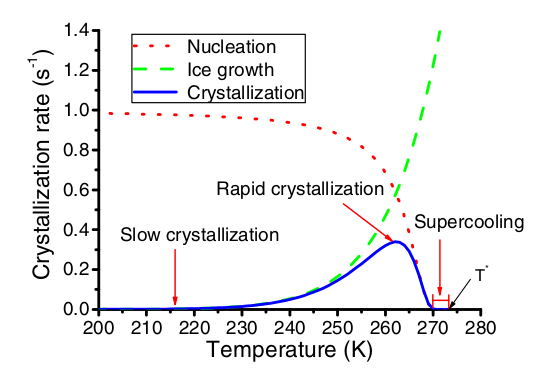
\includegraphics[width=0.6\textwidth]{crystallization_rate.png}
	\caption{Crystallization rate in function of temperature.}	
	\label{2.2fig}
\end{figure} 
\noindent Finally, the coefficient $C_f$ that appears on Equations \ref{2.9} and \ref{2.10} as commented above, is defined for the Lee model as:
\begin{equation}
	\label{2.28}
	C_f=J_{\mathrm{hom}} \cdot V_{l}
\end{equation}
where $V_{l}$ is the volume of water in each cell.

\subsection{Interphase porosity models}

\setlength{\parindent}{0.5cm} Interphase porosity models add an aritificial momentum source over the interface between phases to compute the sink of velocity in the solidified region. Therefore, influencing the behavior of the physics during the process of solidification or melting.

\noindent The model implemented in OpenFOAM is \textit{Voller Prakash method} \cite{voller_prakash_1987}, and it defines the source terms, \textit{$S_y$} and \textit{$S_z$} such that when along the fluid domain these terms take on a value of zero, the momentum equations are driven by the actual values of the velocities. On the other side, when it comes to treat the mushy region (i.e. porous region), the value of these source terms dominate convective, diffusive and transient terms and the momentum equation tends to approximate the Darcy's law.

\noindent The two source terms as specified above,
\begin{equation}
	\left\{\begin{array}{l}
	S_{y}=-A v \\
	S_{z}=-A w
	\end{array}\right.
	\label{2.29}
\end{equation}
Then, to specify a term for the function A, it is used the \textit{Carman-Koseny equation}, which is derived from the Darcy's law. The former expresses the gradient for the pressure as a combination of the velocity, \textbf{u}, and the porosity, $\lambda$. The coefficient \textit{C} depends on the morphology of the medium.
\begin{equation}
	gradP=-\left(\frac{C(1-\lambda)^{2}}{\lambda^{3}}\right) \mathbf{u}
	\label{2.30}
\end{equation}
To avoid division by zero, \textit{q} is added to the equations shown 
\begin{equation}
	A=-\left(\frac{C(1-\lambda)^{2}}{\lambda^{3}+q}\right)
	\label{2.31}
\end{equation}
The source terms $S_{y}$ and $S_{z}$ in \ref{2.29} are added in the Eq. \ref{2.32} and \ref{2.33}. The source term $S_{b}$ corresponds to the body forces of the fluid and will be discussed later on this thesis.
\begin{equation}
	\begin{aligned}
		\frac{\partial(\rho v)}{\partial t}+\operatorname{div}(\rho \mathbf{u} v)=\operatorname{div}(\mu \operatorname{grad} v)-\frac{\partial P}{\partial y}+S_{y} 
	\end{aligned}
	\label{2.32}
\end{equation}
\begin{equation}
	\begin{aligned}
		\frac{\partial(\rho w)}{\partial t}+\operatorname{div}(\rho \mathbf{u} w)=\operatorname{div}(\mu \operatorname{grad} w)-\frac{\partial P}{\partial z}+S_{z}+S_{b}
	\end{aligned}
	\label{2.33}
\end{equation}

\subsubsection{Surface tension model}

\setlength{\parindent}{0.5cm} The surface tension is only specified on a phase pair basis. In this version of OpenFOAM, it is present a constant model for a given $\sigma$.




